%%%%%%%%%%%%%%%%%%%%%%%%%%%%%%%%%%%%%%%%%
% Stylish Article
% LaTeX Template
% Version 2.1 (1/10/15)
%
% This template has been downloaded from:
% http://www.LaTeXTemplates.com
%
% Original author:
% Mathias Legrand (legrand.mathias@gmail.com) 
% With extensive modifications by:
% Vel (vel@latextemplates.com)
%
% License:
% CC BY-NC-SA 3.0 (http://creativecommons.org/licenses/by-nc-sa/3.0/)
%
%%%%%%%%%%%%%%%%%%%%%%%%%%%%%%%%%%%%%%%%%

%----------------------------------------------------------------------------------------
%	PACKAGES AND OTHER DOCUMENT CONFIGURATIONS
%----------------------------------------------------------------------------------------

\documentclass[fleqn,10pt]{SelfArx} % Document font size and equations flushed left

\usepackage[english]{babel} % Specify a different language here - english by default

\usepackage{lipsum} % Required to insert dummy text. To be removed otherwise

%----------------------------------------------------------------------------------------
%	COLUMNS
%----------------------------------------------------------------------------------------

\setlength{\columnsep}{0.55cm} % Distance between the two columns of text
\setlength{\fboxrule}{0.75pt} % Width of the border around the abstract

%----------------------------------------------------------------------------------------
%	COLORS
%----------------------------------------------------------------------------------------

\definecolor{color1}{RGB}{0,0,90} % Color of the article title and sections
\definecolor{color2}{RGB}{0,20,20} % Color of the boxes behind the abstract and headings

%----------------------------------------------------------------------------------------
%	HYPERLINKS
%----------------------------------------------------------------------------------------

\usepackage{hyperref} % Required for hyperlinks
\hypersetup{hidelinks,colorlinks,breaklinks=true,urlcolor=color2,citecolor=color1,linkcolor=color1,bookmarksopen=false,pdftitle={Title},pdfauthor={Author}}

%----------------------------------------------------------------------------------------
%	ARTICLE INFORMATION
%----------------------------------------------------------------------------------------

\JournalInfo{Bla} % Journal information
\Archive{Bla} % Additional notes (e.g. copyright, DOI, review/research article)

\PaperTitle{Testing of ETL} % Article title

\Authors{Alexander Brandborg\textsuperscript{1}, Mathias Claus Jensen\textsuperscript{1}, Mikael Vind Mikkelsen\textsuperscript{1}, Arash Michael Sami Kjær\textsuperscript{1}} % Authors
\affiliation{\textsuperscript{1}\textit{Student at the Department of Computer Science, University of Aalborg, Aalborg, Denmark}} % Author affiliation
%\affiliation{\textsuperscript{2}\textit{Department of Chemistry, University of Examples, London, United Kingdom}} % Author affiliation
%\affiliation{*\textbf{Corresponding author}: john@smith.com} % Corresponding author

\Keywords{Keyword1 --- Keyword2 --- Keyword3} % Keywords - if you don't want any simply remove all the text between the curly brackets
\newcommand{\keywordname}{Keywords} % Defines the keywords heading name

%----------------------------------------------------------------------------------------
%	ABSTRACT
%----------------------------------------------------------------------------------------

\Abstract{The python package pygrametl allows developers to construct ETL systems through an API. We develop a testing framework, \FW{}, which allows testers to evaluate programs developed using pygrametl. The framework is developed for both functional- and regression testing at the system level. It is based on source to target testing. Here an ETL system is tested by asserting about properties of the DW, which it populates. \FW{} can be used to check whether assertions are upheld by such a DW. These assertions are implemented using \FW{}’s predicate classes. These allow testers to assert about DW properties relating to data loss and business rules. After development we evaluate \FW{} against manual testing, where testers write SQL to test for properties. We found that both methods result in test implementations with the same runtime. However, manual testing needed 110 statements for its implementation, where \FW{} only needed 11.}

%----------------------------------------------------------------------------------------

\begin{document}

\flushbottom % Makes all text pages the same height

\maketitle % Print the title and abstract box

\tableofcontents % Print the contents section

\thispagestyle{empty} % Removes page numbering from the first page

%----------------------------------------------------------------------------------------
%	ARTICLE CONTENTS
%----------------------------------------------------------------------------------------

\section{Introduction}\label{intro} % The \section*{} command stops section numbering
%\addcontentsline{toc}{section}{Introduction} % Adds this section to the table of contents
To make sure that a piece of software can be expected to run at low risk of failure, it must be tested. Today we have specialized software that assist in the automatic execution of tests. This allows testers to focus more on what to test and less on test implementation. Conceptually this should lead to tests of a higher quality.

Some testing tools such as JUnit have a broad application, while other test frameworks have a more specific use. Per extension, there exists many tools exclusively used for testing Extract-Transform-Load (ETL) systems. These systems support the creation and update of data warehouses (DW), which are mainly used for business analysis. An ETL process will extract data from a set of sources, apply transformations to that data and then load it into a DW. Often GUI-based tools are used, when developing ETL systems. The pygrametl python package, which is open source, allows for coding entire ETL systems instead. The idea being that experts perform better when using an API rather than a GUI \cite{thomsen2009pygrametl}. Our goal for this article is to develop a testing framework, which may assist users of pygrametl in testing their ETL systems.

ETL testing may be set up manually using SQL. Yet, in the current market many different testing tools exists. These allow for the automation of tests. Testing often occurs by focusing on the DW, which the ETL system populates. QuerySurge\cite{QuerySurge} for example, focuses on comparing the data from sources to the data in the DW. The tool is build on the idea that data is often unaltered, as it passes through the ETL process. This means that column A in a source must be one-to-one mappable to column B in the DW. Testing of this type only requires the user to supply some simple mappings between sources and DW. As such, QuerySurge presents itself as novice-friendly and allows for testing through a GUI. Yet, if mappings between source data and DW become more complex, testers will need to write up some SQL code. We determine that this kind of tool is not fitting for the users of pygrametl. As pygrametl users are experts, they will not gain anything from the novice-friendly features of QuerySurge. The amount of code needed for testing may also be rather large, if there is a frequent need for writing SQL.

Testing may also occur through the comparison of tables within a populated DW to those defined by the user. By writing up a table, testers assert, how they expect a DW table to look after load. The truth value of this assertion can be found by comparing to the actual DW table. For this, tools such as AnyDBTest\cite{AnyDbTest} may be used. AnyDBTest also allows testers to describe, what kind of comparison should be made. For example, we may test that one table is the subset of another. Our issue with this type of testing requires the setup of many user-defined tables. Again a large amount of test code needs to be written. We do however believe that table comparison is a powerful tool for ETL testing. Yet, comparison between tables should not be the only assertable property of a DW.

Having looked at some of the currently available tools, we find that they require a lot of test code to be written. To get a wider test coverage, we need to decrease the amount of code necessary for each test. We also fear that faults may be more likely to occur in the test code, as it grows larger. Such faults can undermine the usefulness and accuracy of test results.

To allow for automated testing of pygrametl programs, we have developed \FW{}. Like AnyDBTest it is assertion-based. However, it does not only allow for assertions to be made upon the relationships of tables. Assertions may relate to other DW properties such as data integrity. The framework allows for functional testing at the system level, once all components of the ETL have been integrated. As the framework automates test execution, it can also be used for regression testing. We aim to help testers in writing less code for a single test. This should lead to less time spend on each test, enabling a wider coverage during testing. Covering more of the software should increase its overall quality. We also need for the tests to be executed at a reasonable speed. If the tests are quick to write, but slow to execute, users may fall back on other tools or perform testing manually.

The rest of this paper is organized as follows. \Cref{sect:RelatedWorks} will give a brief overview of some related literature. This is followed by an introduction to the pygrametl python package in \cref{sect:pygrametl}. \Cref{sect:btesting} will explain some basic testing terminology relevant to the paper. This leads into an overview of \FW{} in \cref{sect:Overview}, followed by some sections describing its implementation. \Cref{sec:dwpopulator} shows how the framework allows for dynamic replacement of sources and DW in a pygrametl program.  In \cref{sect:interdatarep} we describe the classes used to represent the DW during testing. Afterwards, \cref{sect:pred} explains the different types of predicates, used to assert properties of a DW. After implementation \cref{sect:eval} will focus on evaluating the framework. Finally, in \cref{sect:conc} we conclude upon the framework.




%------------------------------------------------

\section{Methods}

\begin{figure*}[ht]\centering % Using \begin{figure*} makes the figure take up the entire width of the page
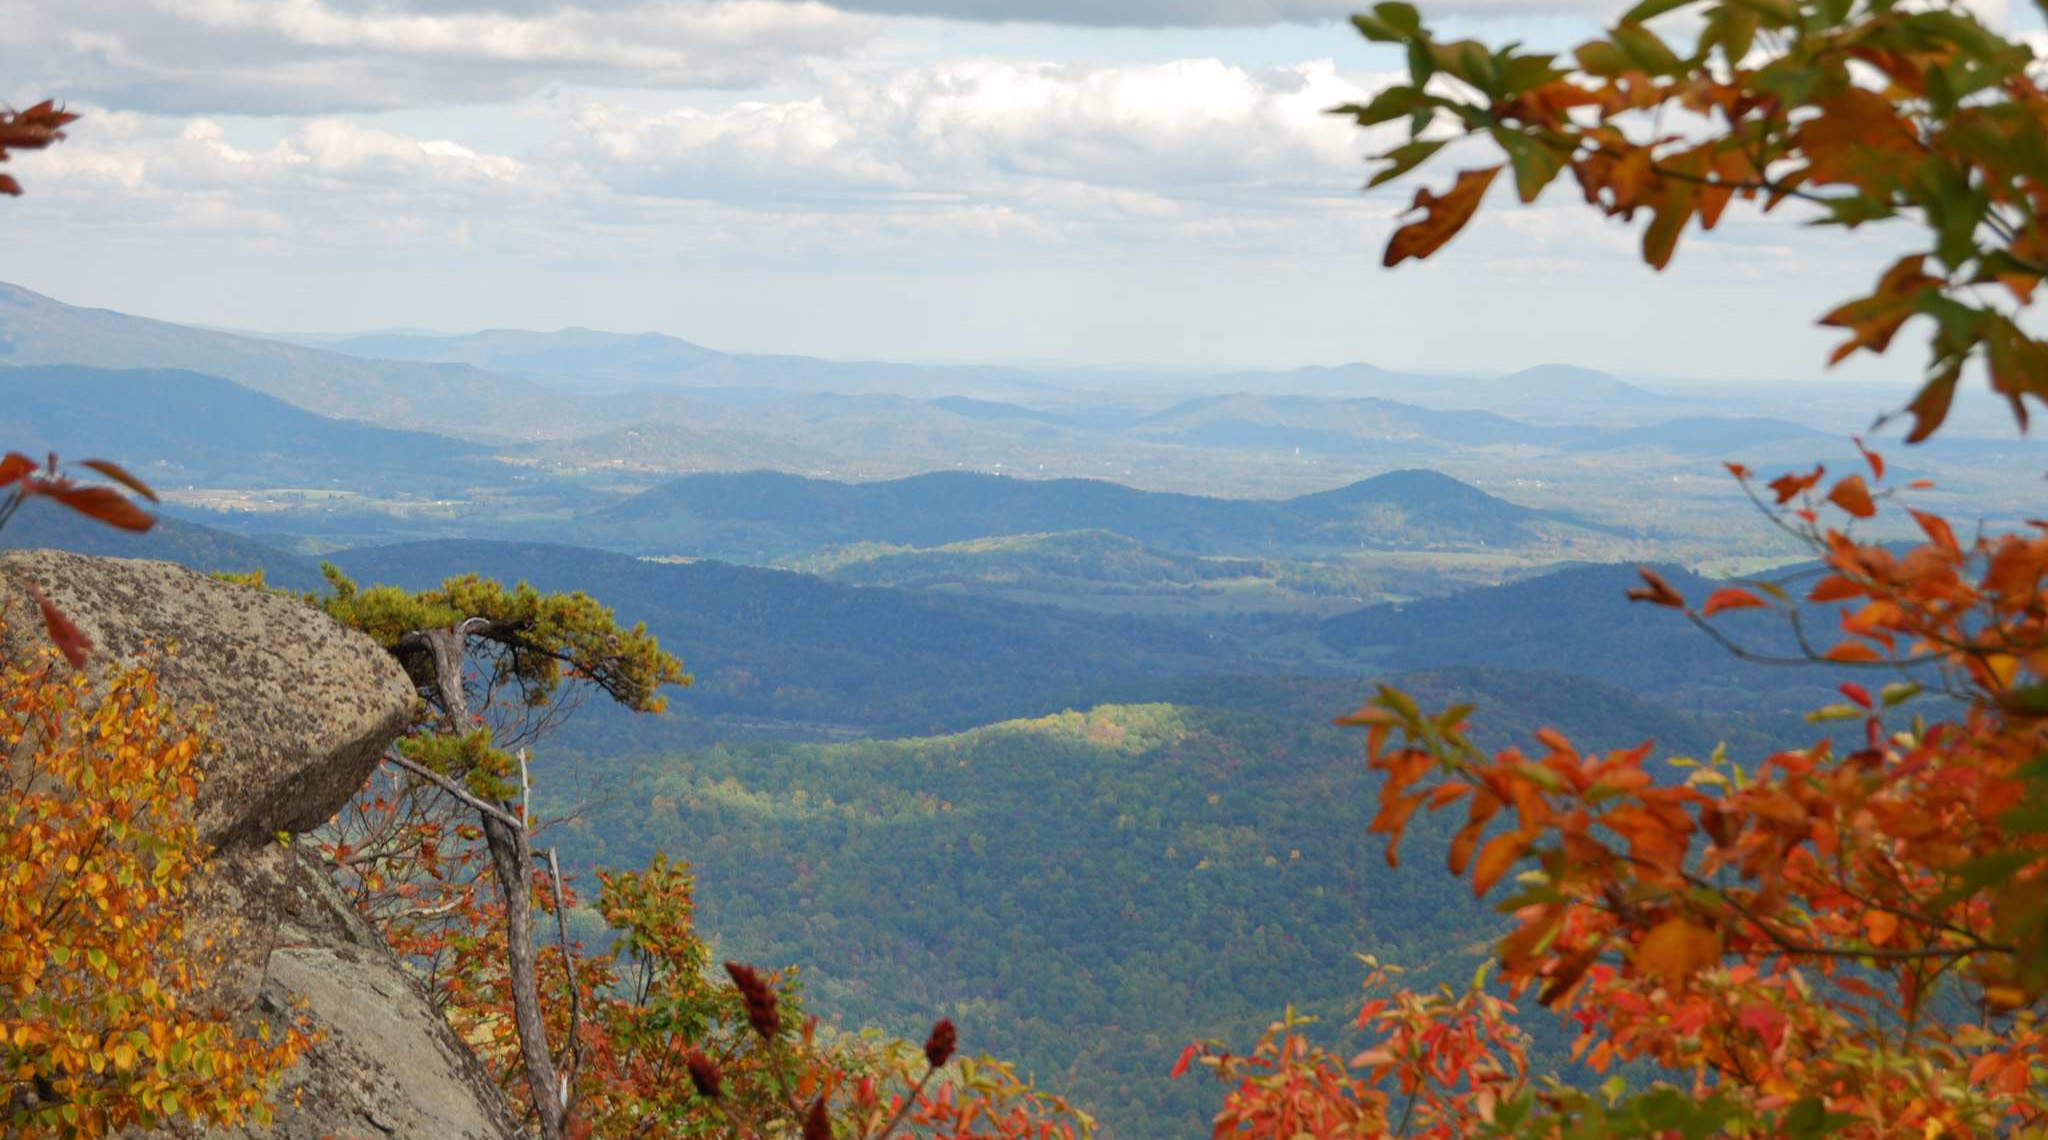
\includegraphics[width=\linewidth]{figures/view}
\caption{Wide Picture}
\label{fig:view}
\end{figure*}

\lipsum[4] % Dummy text

\begin{equation}
\cos^3 \theta =\frac{1}{4}\cos\theta+\frac{3}{4}\cos 3\theta
\label{eq:refname2}
\end{equation}

\lipsum[5] % Dummy text

\begin{enumerate}[noitemsep] % [noitemsep] removes whitespace between the items for a compact look
\item First item in a list
\item Second item in a list
\item Third item in a list
\end{enumerate}

\subsection{Subsection}

\lipsum[6] % Dummy text

\paragraph{Paragraph} \lipsum[7] % Dummy text
\paragraph{Paragraph} \lipsum[8] % Dummy text

\subsection{Subsection}

\lipsum[9] % Dummy text

\begin{figure}[ht]\centering
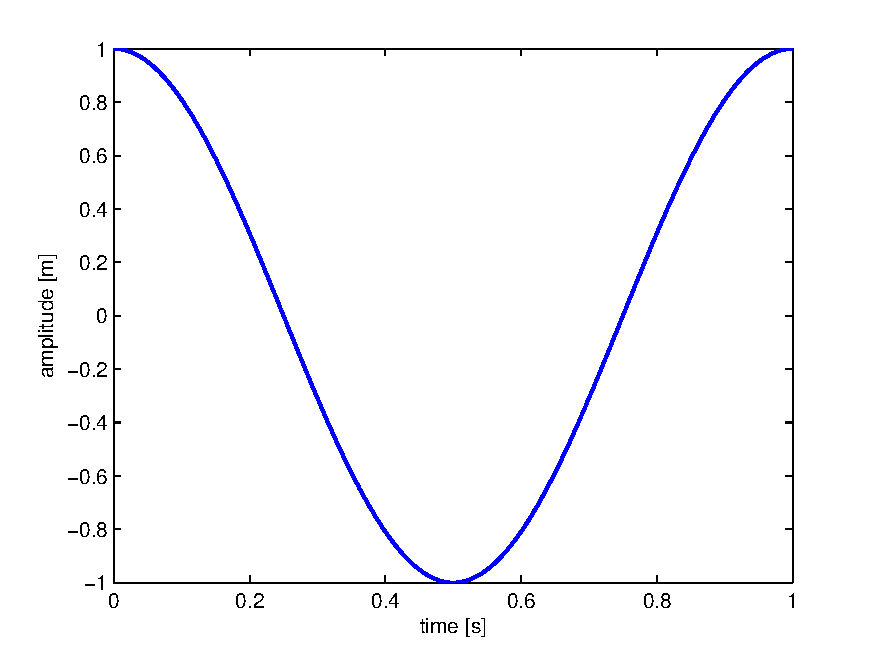
\includegraphics[width=\linewidth]{figures/results}
\caption{In-text Picture}
\label{fig:results}
\end{figure}

Reference to Figure \ref{fig:results}.

%------------------------------------------------

\section{Results and Discussion}

\lipsum[10] % Dummy text

\subsection{Subsection}

\lipsum[11] % Dummy text

\begin{table}[hbt]
\caption{Table of Grades}
\centering
\begin{tabular}{llr}
\toprule
\multicolumn{2}{c}{Name} \\
\cmidrule(r){1-2}
First name & Last Name & Grade \\
\midrule
John & Doe & $7.5$ \\
Richard & Miles & $2$ \\
\bottomrule
\end{tabular}
\label{tab:label}
\end{table}

\subsubsection{Subsubsection}

\lipsum[12] % Dummy text

\begin{description}
\item[Word] Definition
\item[Concept] Explanation
\item[Idea] Text
\end{description}

\subsubsection{Subsubsection}

\lipsum[13] % Dummy text

\begin{itemize}[noitemsep] % [noitemsep] removes whitespace between the items for a compact look
\item First item in a list
\item Second item in a list
\item Third item in a list
\end{itemize}

\subsubsection{Subsubsection}

\lipsum[14] % Dummy text

\subsection{Subsection}

\lipsum[15-23] % Dummy text

%------------------------------------------------

\phantomsection % Nessesary for hyperref to jump to the correct page

\section*{Acknowledgments} % The \section*{} command stops section numbering

\addcontentsline{toc}{section}{Acknowledgments} % Adds this section to the table of contents

Thanks to Marcus Aurelius, the true Emperor and protector of Philosophy, for teaching me that my happiness does not depend on outside events, of which I have no control, but rather my own mind, of which I have power over.r=color1,bookmarksopen=false,pdftitle={Title},pdfauthor={Author}}

%--------------------------------------------------------------

Thanks to Bruce Willis, who visited me once in a dream and said he would call me in real life, which he did not. He was also pretty cool in Predator.


%----------------------------------------------------------------------------------------
%	REFERENCE LIST
%----------------------------------------------------------------------------------------
\phantomsection % Nessesary for hyperref to jump to the correct page
\bibliographystyle{unsrt}
\bibliography{sample}

%----------------------------------------------------------------------------------------

\end{document}